\chapter{Propuesta Pedagógica}

En este capítulo pasamos a detallar la ventaja pedagógica que se pretende obtener en en base a los objetivos que presentamos en el segundo capítulo y a los antecedentes vistos en el tercero.

\section{Análisis general del problema}

La enseñanza de la programación suele considerarse bastante complicada, ``ya que muchos estudiantes encuentran bastantes dificultades cuando empiezan a programar'' (\cite{rubio_uso_2018}), de hecho ``La existencia de altas tasas de fracaso y la subsiguiente incapacidad de los estudiantes para escribir programas simples al final de una unidad de programación son solo dos de los problemas que inciden en las facultades de informática todo el mundo'' (\cite{bruce_contemporary_nodate}).

\bigskip
Aun así la programación es uno de los pilares mas importantes de la informática, por lo que su aprendizaje es de carácter obligatorio para todo el mundo. De hecho en muchos países como Finlandia, Alemania y Estonia promueven el aprendizaje de programación desde la educación primaria, en nuestro país El estudio de las CC en Educación Primaria y Secundaria se encuentra en su fase inicial y se ha
empezado a introducir recientemente por lo que aún no ha sido adoptado por la mayoría de centros escolares. Como resultado, el número de niños y niñas que a día de hoy estudian ciencias de la computación es
todavía una minoría (\cite{fecyt_educacion_2016}) pero se está promoviendo el aprendizaje a edades cada vez más tempranas.

\bigskip
Para enseñar programación a nuestros alumnos tenemos que tener en cuenta las dificultades que suponen la interacción ordenador/alumno y ``contar con una actitud receptiva a los problemas que les plantea a los alumnos la introducción de un lenguaje formal y su uso para programar y resolver problemas'' \cite{vitale_psycopedagogical_1990}.

\section{Análisis de las soluciones existentes}

Tras analizar las tres soluciones libres descritas en los antecedentes (Coderunner, Python Tutor y Jupyter Notebooks) hemos encontrado que las tres tienen el mismo problema. En todos los casos nuestros alumnos tienen que aprender a usar una herramienta concreta que posiblemente no vayan a volver a utilizar en su futuro profesional. Esto sería comparable a lo que didácticamente decimos que el alumno ``aprende a aprobar exámenes'' mas que aprender los contenidos de la asignatura. Por esto, nos gustaría proponer una metodología donde los alumnos usen herramientas que van a tener que usar en futuro profesional (o académico) como pueden ser un sistema de control de versiones así como sistemas de integración continua, o \textit{continuous integration (CI)}.

\section {Temario relacionado con la programación informática}

Tal y como indica el Decreto 110-2016. Las tecnologías de la información y de la comunicación para el aprendizaje y el conocimiento se utilizarán de manera habitual como herramientas integradas para el desarrollo del currículo. Asimismo en los currículos de las distintas ramas educativos donde podemos ejercer como profesores incluyen asignaturas relacionadas con la informática y de forma más específica con la programación informática.

\subsection {Bachillerato}

En la Orden de 14 de julio de 2016 se especifica el currículo de

Según la legislación Tecnologías de la Información y de la Comunicación

\subsection {Ciclo Formativo Grado Medio}

La Orden EDU/2187/2009, de. 3 de Julio establece el currículo del ciclo formativo de Grado Medio correspondiente al título de ``Técnico en Sistemas Microinformáticos y Redes (SMR)'' que es el único ciclo de grado medio relacionado con la informática donde la única asignatura ligeramente relacionada con la programación es ``Aplicaciones web'', pero dicha asignatura se centra más en el despliegue de aplicaciones que en la programación en sí, por lo que aunque nuestra metodología se podría adaptar para enseñar a configurar como desplegar aplicaciones web no entra dentro del alcance de este trabajo por lo que se deja como posible trabajo futuro.

\subsection {Ciclo Formativo Grado Superior}

Existen tres ciclos formativos de grado superior del plan LOE relacionados con la informática, la Orden EDU/392/2010, de 20 de enero, por la que se establece el currículo del ciclo formativo de Grado Superior correspondiente al título de ``Técnico Superior en Administración de Sistemas Informáticos en Red'' describe las asignaturas ``Lenguajes de Marca y Sistemas de Gestión de Información'' y ``Gestión de Bases de Datos'' en las que nuestra metodología se puede aplicar para corregir los ejercicios ya que se enseñan los lenguajes HTML, SQL, Javascript, XML así como algunos subconjuntos de XML como son DTD y XSD. Los currículos del título de ``Técnico Superior en Desarrollo de Aplicaciones Web'' definido en la Orden EDU/2887/2010, de 2 de noviembre y el de ``Técnico Superior en Desarrollo de Aplicaciones Multiplataforma'' definido en la Orden EDU/2000/2010, de 13 de julio definen varias asignaturas, algunas comunes, como pueden ser ``Programación'', ``Bases de Datos'' y ``Lenguajes de marcas y sistemas de gestión de información'' y otras específicas de cada título como pueden ser ``Programación multimedia y dispositivos móviles'' o ``Desarrollo web en entorno cliente'' que están centradas en el aprendizaje de la programación informática y en los que si encajaría nuestra metodología.


\subsection {Formación Profesional Básica}

La Orden ECD/1030/2014, de 11 de junio define el ``Título Profesional Básico en Informática y Comunicaciones'' y la Orden ECD/1633/2014, de 11 de septiembre define el  ``Título Profesional Básico en Informática de Oficina'', siendo ambas titulaciones las únicas relacionadas con la informática de todas las que componen la formación profesional básica, pero al igual que con el ciclo formativo de Grado Medio ambos currículos carecen de temario específico de programación por lo que queda fuera del ámbito de este proyecto.


\section{Encuesta de percepción}

Se realizó una pequeña encuesta con varios profesores de diferentes ámbitos con el fin de ver si nuestra hipótesis de que la corrección de ejercicios era la parte mas tediosa que realizaban como docentes.

\begin{figure}[h!]
\centering
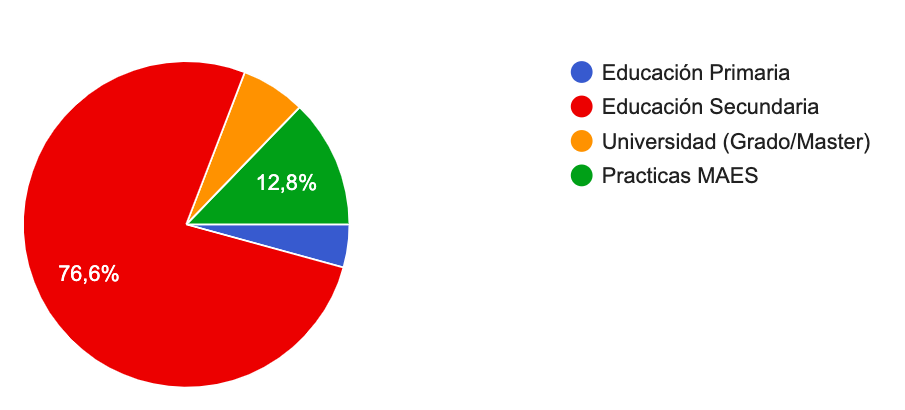
\includegraphics[width=1.0\textwidth]{../images/quiz_1}
\caption{¿Dónde sueles impartir tus clases?}
\label{fig:quiz_1}
\end{figure}

\begin{figure}[h!]
\centering
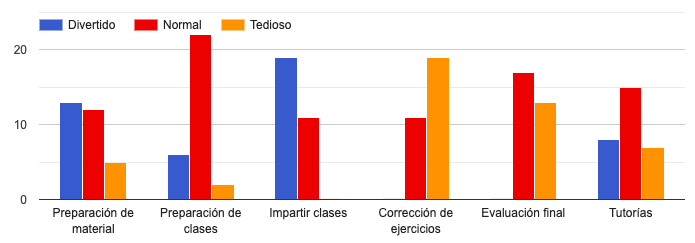
\includegraphics[width=1.0\textwidth]{../images/quiz_2}
\caption{Valora las siguientes tareas que sueles realizar}
\label{fig:quiz_2}
\end{figure}


\begin{figure}[h!]
\centering
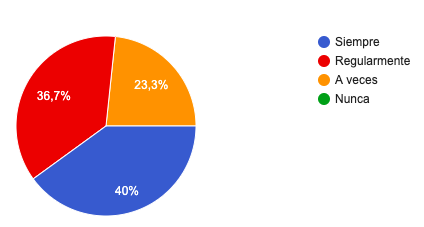
\includegraphics[width=1.0\textwidth]{../images/quiz_3}
\caption{¿Elaboras tus propios ejercicios?}
\label{fig:quiz_3}
\end{figure}



\begin{figure}[h!]
\centering
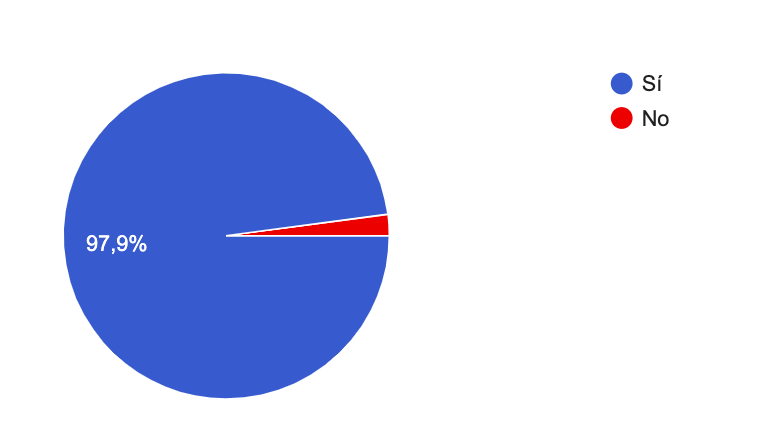
\includegraphics[width=1.0\textwidth]{../images/quiz_4}
\caption{¿Sueles entregar correcciones de los ejercicios?}
\label{fig:quiz_4}
\end{figure}


\section{Metodología propuesta}


\subsection{Objetivos}

El objetivo de nuestra metodología es enseñar programación de una forma diferente, con ejercicios, autocorrección y con tecnologías que se usan en el día a día de cualquier informático que se dedique profesionalmente a ello. Para ello FALTA TEXTO

\subsection{Contenidos}

\subsection{Competencias}

\subsection{Temporización}




